\documentclass[handout]{beamer}
%\documentclass{beamer}
\usepackage{tikz}
\usepackage{multicol}
\usepackage{lmodern}
\usepackage[linesnumbered,ruled]{algorithm2e}

\usetheme{CambridgeUS}
\graphicspath{{/Users/benjamindraves/Desktop/figures}}

\makeatletter
\setbeamertemplate{footline}
{
  \leavevmode%
  \hbox{%
  \begin{beamercolorbox}[wd=.7\paperwidth,ht=2.25ex,dp=1ex,center]{author in head/foot}%
    \usebeamerfont{author in head/foot}\insertshortauthor~~\beamer@ifempty{\insertshortinstitute}{}{(\insertshortinstitute)}
  \end{beamercolorbox}%
  \begin{beamercolorbox}[wd=.3\paperwidth,ht=2.25ex,dp=1ex,center]{date in head/foot}%
    \usebeamerfont{date in head/foot}\insertshorttitle{}
  \end{beamercolorbox}}%
  \vskip0pt%
}
\makeatother
\title{Latent Networks Models}
\subtitle{Game of Thrones}
\author{Lily Chou, Ben Draves, Nathan Josephs, Kelly Kung}
\date{December 12, 2018}
\institute[Boston University] 
{
  Department of Mathematics and Statistics\\
  Boston University
  }
\date{\today}
\subject{Latent Vector Network Models}

\begin{document}


%-------------------------------------------------
%
%           Introduction + Background
%
%-------------------------------------------------
\begin{frame}
  \titlepage
\end{frame}
\begin{frame}
\frametitle{Overview}
\tableofcontents
\end{frame}

\section{Introduction}
\begin{frame}
 \frametitle{Data}
\begin{enumerate}
\item Data origin: A Song of Ice and Fire $\cdot$ A storm of Swords
\item Data form: 352 pairs of characters and the number of interaction between them
\end{enumerate}

We start our analysis by constructing a Weighted Network $G$: 
\begin{enumerate}[i]
\item Characters $\rightarrow$ nodes 
\:  $N_V (G)= 107$
\item Interactions $\rightarrow$ edges   
\: $N_E (G) = 352$
\item numbers of interaction $\rightarrow$ Weights on the edge
\end{enumerate}
\end{frame}

\begin{frame}
\frametitle{Form a Network}
% \includegraphics[width = 0.75\textwidth]{{"initial_net"}.pdf}
PICTURE HERE
\begin{enumerate}[a]
\item Q: How to handle the sparsity of the network? 
\item A: Take a subnetwork of G, cut off at 100 interactions, call it G'
\item $N_V (G')= 24$, $N_E (G') = 102$
\item Use adjacency matrix A to represent G': 
 \begin{enumerate}[i]
  \item $a(i, j)$ = number of interactions between $i$th and $j$th character
  \item  i.e., $a(i, j) = 0$ if there's no interaction between the two people
 \end{enumerate}
\end{enumerate}
\end{frame} 



%-------------------------------------------------
%
%           Model Section
%
%-------------------------------------------------

\section{Latent Network Model}
\begin{frame}{Latent Network Model}
Using Hoff's work, we model the presence of an edge given our latent variables as
\[\text{logit} \ \mathbb{P}(Y_{ij} = 1|Z) = ||Z_i - Z_j|| + \epsilon_{ij}\]

where $||Z_i - Z_j||$ is the latent distance between nodes $i$ and $j$ and 
\[Z_i \overset{ind}{\sim}\sum_{k=1}^G \lambda_k\text{MVN}_d(\mu_k,\sigma_k^2I_d)\]

\end{frame}

\begin{frame}{Latent Network Model: Priors}
\begin{align*}
Y_{ij} | Z_i, Z_j &\overset{ind}\sim \text{Bern}\Big[\text{logit}^{-1}\big(\Vert Z_i - Z_j \Vert\big)\Big] \\
Z_i | K_i = k_i &\overset{ind}\sim MVN(\mu_{k_i}, \sigma_{k_i}^2 I_d) \\
K &\overset{iid}\sim \text{Multinoulli}\big(G, \lambda \big) \\
\lambda_k &\overset{iid}\sim \frac{1}{G} \\
\mu_k &\overset{iid}\sim \text{MVN}_d(0, I_2) \\
\sigma_k^2 &\overset{iid}\sim \text{Inv} \chi^2_1
\end{align*}
\end{frame}

\begingroup
\small
\begin{frame}{Latent Network Model: Likelihood}
\begin{align*}
\onslide<1->{\mathcal{L}(Z, \theta; Y) &= \prod_{i<j}\mathbb{P}(Y_{ij} | Z_i, Z_j) \mathbb{P}(Z_i | K_i, \mu_{k_i}, \sigma_{k_i}^2) \mathbb{P}(Z_j | K_j, \mu_{k_j}, \sigma_j^2) \\ 
&\ \ \ \ \ \ \ \ \times  \mathbb{P}(K_i | \lambda_i) \mathbb{P}(\lambda_i)\mathbb{P}(\mu_{k_i})\mathbb{P}(\sigma_{k_i}^2)\mathbb{P}(K_j)\mathbb{P}(\mu_{k_j})\mathbb{P}(\sigma_{k_j}^2) \\}
\onslide<2->{&\propto \prod_{i<j}\Big(\text{logit}^{-1}\big(\Vert Z_i-Z_j\Vert)\Big)^{Y_{ij}}\Big(1 - \text{logit}^{-1}\big(\Vert Z_i-Z_j\Vert)\Big)^{1 - Y_{ij}} \\
& \times \frac{1}{(\sigma_{k_i}^2)^{1/2}}\exp\Big\{-\frac{1}{2\sigma_{k_i}^2}(Z_i - \mu_{k_i})^T( Z_i - \mu_{k_i}) \Big\} \enspace \frac{1}{(\sigma_{k_j}^2)^{1/2}}\\
&\times\exp\Big\{-\frac{1}{2\sigma_{k_j}^2}(Z_j - \mu_{k_j})^T (Z_j - \mu_{k_j})\Big\}  \exp\Big\{-\frac{1}{2}\mu_{k_i}^T\mu_{k_i}\Big\}\\
&\times \exp\Big\{-\frac{1}{2}\mu_{k_j}^T\mu_{k_j}\Big\}  \times \frac{1}{(\sigma_{k_i}^2)^2}\exp\Big\{-\frac{1}{\sigma_{k_i}^2}\Big\}\frac{1}{(\sigma_{k_j}^2)^2}\exp\Big\{-\frac{1}{\sigma_{k_j}^2}\Big\} \\
&\times \lambda_i \times \lambda_j}
\end{align*}
\end{frame}
\endgroup

%-------------------------------------------------
%
%           Expectation Maximization
%
%-------------------------------------------------

\section{Expectaction Maximimation}


\subsection{Unweighted Network Model}
\begin{frame}{Unweighted Network Model}
Let $Y_{ij}$ indicate whether there is an edge $E_{ij}$ between nodes $i$ and $j$.
\begin{align*}
Y_{ij} | p_{ij} &\overset{ind}\sim \text{Bern}(p_{ij}) \\
p_{ij} &\overset{iid}\sim \text{Beta}(\alpha, \beta)
\end{align*}
where $p_{ij} \equiv 2-2*\text{logit}^{-1} (d_{ij})$. \newline

Then the log-likelihood for this model can be written as
\begin{align*}
l(p, \alpha, \beta ; Y) &= \sum_{i<j} Y_{ij}\log \Big(\frac{p_{ij}}{1 - p_{ij}}\Big) + \log(1-p_{ij})  + \log \Gamma(\alpha + \beta) \\
&- \log \Gamma(\alpha) - \log \Gamma(\beta) + (\alpha - 1)\log p_{ij} + (\beta - 1)\log(1 - p_{ij})
\end{align*}
\end{frame}

\begin{frame}{Unweighted Network Model: E-Step}
We can take the expectation of the log-likelihood given the data \textbf{Y} and parameters $\theta = (\alpha, \beta)$
\begin{align*}
Q\big(\theta; \theta^{(t)}\big) &= \sum_{i<j} (Y_{ij} + \alpha - 1) \mathbb{E}_{p_{ij} | Y_{ij}, \theta^{(t)}} [\log  p_{ij}] \\
&+ (\beta -Y_{ij}) \mathbb{E}_{p_{ij} | Y_{ij}, \theta^{(t)}} \big[\log (1-p_{ij})\big] + \log \Gamma(\alpha + \beta) \\
&- \log \Gamma(\alpha) - \log \Gamma(\beta) 
\end{align*}

Since $p_{ij}|Y_{ij}, \theta \propto Beta(\alpha + Y_{ij}, \beta + 1 - Y_{ij})$, we define the following 
\begin{align*}
\pi_{ij} &\equiv \mathbb{E}_{p_{ij} | Y_{ij}, \theta} \big[\log p_{ij}\big] = \Psi\Big(\alpha + Y_{ij}\Big) - \Psi\Big(\alpha + \beta + 1\Big) \\
\eta_{ij} &\equiv \mathbb{E}_{p_{ij} | Y_{ij}, \theta} \big[\log (1 - p_{ij})\big] = \Psi\Big(\beta + 1 - Y_{ij}\Big) - \Psi\Big(\alpha + \beta + 1\Big)
\end{align*}
\end{frame}

\begin{frame}{Unweighted Network Model: M-Step}
To maximize, $Q(\theta, \theta^{(t)})$ with respect to $\theta$, we see that $\theta^{(t+1)}$ must satisfy the following:
\begin{align*}
\Psi\Big(\alpha^{(t+1)} + \beta^{(t)}\Big) - \Psi(\alpha^{(t+1)}) &= -\frac{\sum_{i<n}\mathbb{E}_{p_{ij} | Y_{ij}, \theta^{(t)}} \big[\log p_{ij}\big]}{{n \choose 2}} \tag{$\alpha_U$}\\
\Psi\Big(\alpha^{(t+1)} + \beta^{(t+1)}\Big) - \Psi(\beta^{(t+1)}) &= -\frac{\sum_{i<n}\mathbb{E}_{p_{ij} | Y_{ij}, \theta^{(t)}} \big[\log (1 - p_{ij})\big]}{{n \choose 2}} \tag{$\beta_U$}
\end{align*}

Here, we use Newton-Raphson to obtain both $\alpha^{(t+1)}$ and $\beta^{(t+1)}$.
\end{frame}

\begin{frame}{Unweighted Network Model: Pseudocode}
\begin{center}
\scalebox{.9}{  
    \begin{algorithm*}[H]
    \SetKwInOut{Input}{Input}
    \SetKwInOut{Output}{Output}
    \underline{LNM EM} $(G, tol)$\;
    \Input{Graph $G$ \\ Tolerance $tol$}
    \Output{Nuisance Parameters $\alpha^*$, $\beta^*$ \\ Latent Probability Estimates $\hat{p}$ \\ Latent Distance Estimates $\hat{d}$}
    Initialize $Q^{(0)}$
    \Repeat{$\vert\frac{Q(\theta^{(t+1)}, \theta^{(t)}) - Q(\theta^{(t)}, \theta^{(t)})}{Q(\theta^{(t)}, \theta^{(t)})}\vert < tol$}{
     \textbf{E:} calculate $\pi^{(t)}$, $\eta^{(t)}$\;
     \textbf{M:}
     update $\alpha^{(t+1)}$ using ($\alpha_U$)\;
     update $\beta^{(t+1)}$ using ($\beta_U$)\;

     calculate $Q(\theta, \theta^{(t+1)})$ 
     }
     \Return $\alpha^*$, $\beta^*$, $\hat{p} =  e^{\pi^*}$, $\hat{d} = logit^{-1}(1 - \frac{e^{\pi^*}}{2})$; where $\alpha^*, \beta^*, \pi^*$ are converged values \
    \caption{EM for simplified latent network unweighted model}
\end{algorithm*}
}
\end{center}
\end{frame}

\begin{frame}{Unweighted Network Model: Distances}
\begin{figure}
    \centering
    %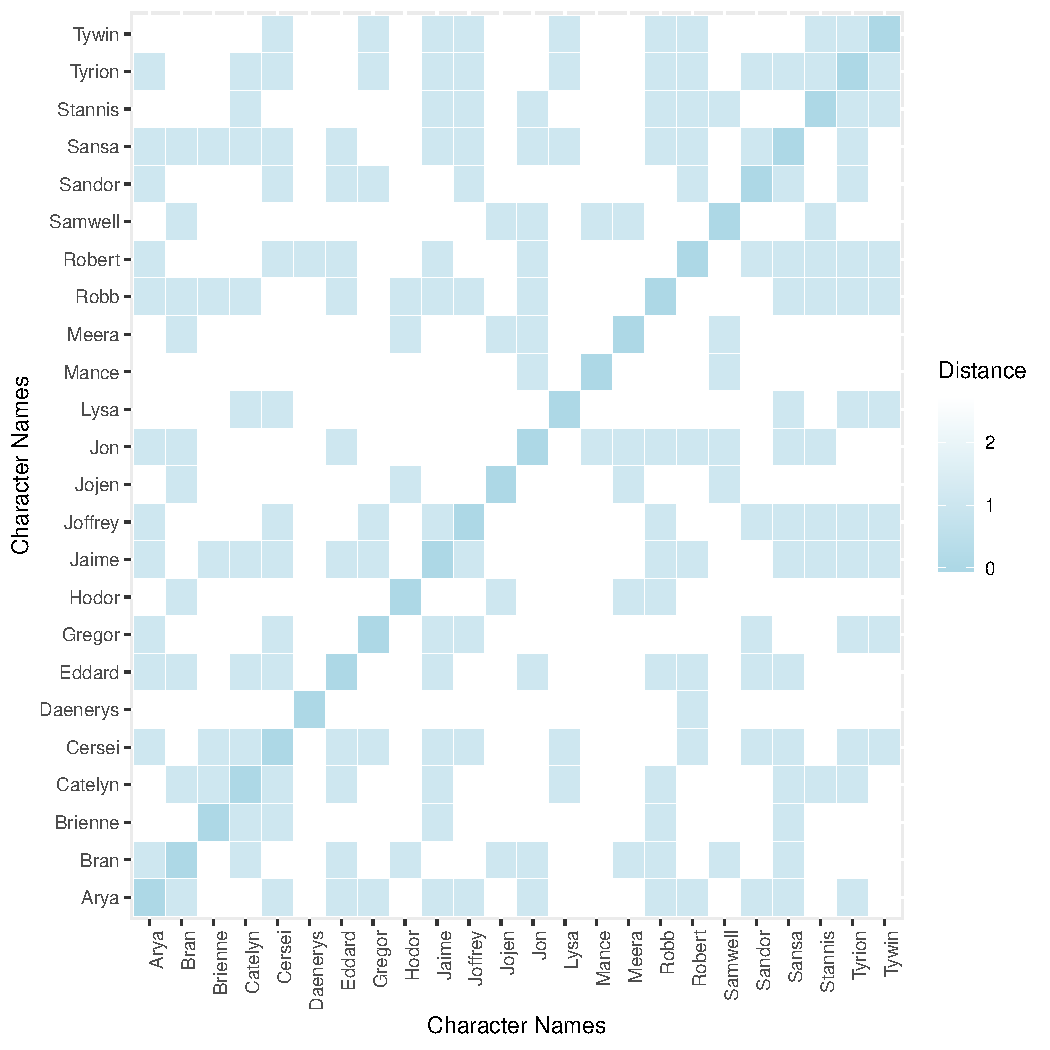
\includegraphics[width = 0.75\textwidth]{heatmap_dist_unweighted.pdf}
    \end{figure}
\end{frame}

\begin{frame}{Unweighted Network Model: Probabilities}
\begin{figure}
    \centering
    %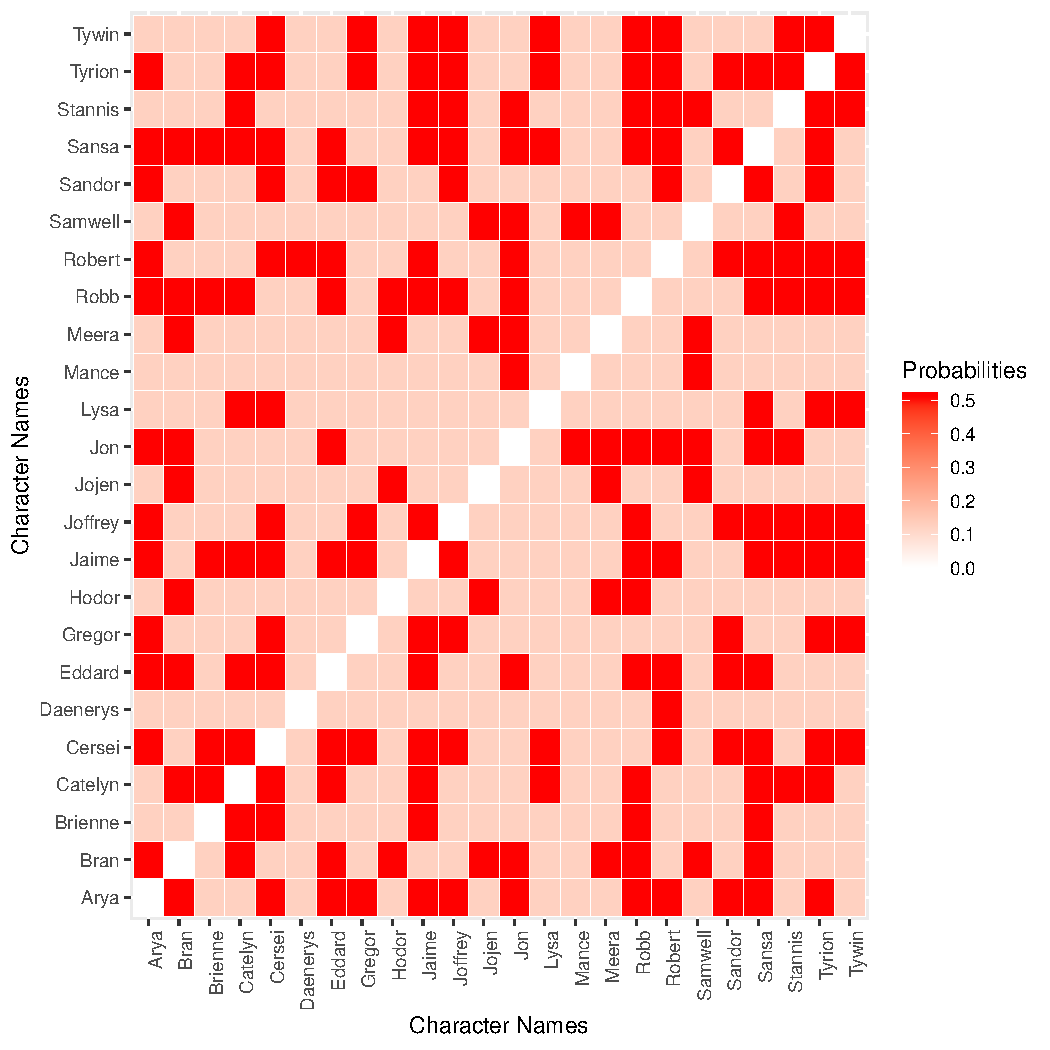
\includegraphics[width = 0.75\textwidth]{heatmap_p_unweighted.pdf}
    \end{figure}
\end{frame}

\subsection{Weighted Network Model}

\begin{frame}{Weighted Network Model}
Let $Y_{ij}$ be the weight on edge $E_{ij}\in \mathbf{E}$.     
    \begin{align*}
    Y_{ij} | \lambda_{ij} &\overset{ind}\sim \text{Pois}(\lambda_{ij}) \\
    \lambda_{ij} &\overset{iid}\sim \text{Gamma}(\alpha, \beta)
\end{align*}
Then the log-likelihood for this model can be written as 
\begin{align*}
l(\lambda, \alpha, \beta ; Y) &= \sum_{i<j}\Big\{ \log \lambda_{ij}\big(Y_{ij} + \alpha - 1) - \lambda_{ij}(1+ \beta)\\
 &-\log(Y_{ij}!) + \alpha \log(\beta) - \log \Gamma(\alpha)\Big\}
\end{align*}
\end{frame}

\begin{frame}{Weighted Network Model: E-Step}
Taking an expectation of this log-likelihood given the data $\mathbf{Y}$ and parameters $\theta = (\alpha, \beta)$ 
\begin{align*}
Q(\theta; \theta^{(t)})  &= \sum_{i<j}\Big\{ (Y_{ij}+ \alpha - 1)\mathbb{E}_{\lambda_{ij}|Y_{ij}, \theta^{(t)}} \big[\log \lambda_{ij}\big] \\
    &- (1+ \beta)\mathbb{E}_{\lambda_{ij}|Y_{ij}, \theta^{(t)}}\big[\lambda_{ij}\big] -\log(Y_{ij}!) + \alpha \log(\beta) - \log \Gamma(\alpha)\Big\}
\end{align*}\pause

Seeing as $\lambda_{ij}|Y_{ij}, \theta \propto \text{Gamma}(\alpha + Y_{ij}, \beta + 1)$  we can define 

\begin{align*}
\pi_{ij} &\equiv \mathbb{E}_{\lambda_{ij}|Y_{ij}, \theta}\big[\lambda_{ij} \big] = \frac{\alpha + Y_{ij}}{1+ \beta} \\
\eta_{ij} &\equiv \mathbb{E}_{\lambda_{ij}|Y_{ij}, \theta}\big[\log \lambda_{ij} \big] = \log(1 + \beta) + \Psi (\alpha + Y_{ij})
\end{align*}

\end{frame}

\begin{frame}{Weighted Network Model: M-Step}
Maximizing $Q(\theta, \theta^{(t)})$ with respect to $\theta$, we see that $\theta^{(t+1)}$ must satisfy 
\begin{align*}
\beta^{(t+1)} &= \frac{\binom{n}{2}}{\sum_{i<j}\pi_{ij}}\alpha^{(t+1)}\\
\Psi(\alpha^{(t+1)}) &= \frac{\sum_{i<j} \eta_{ij} + \binom{n}{2} \log(\beta^{(t+1)})}{\binom{n}{2}} 
\end{align*}
We first update $\beta^{(t+1)}$ using $\alpha^{(t)}$ then use Netwon-Raphson to attain $\theta^{(t+1)}$. 
\end{frame}

\begin{frame}{Weighted Network Model: Psuedo-Code}
\begin{center}
\scalebox{.9}{  
    \begin{algorithm*}[H]
        \SetKwInOut{Input}{Input}
        \SetKwInOut{Output}{Output}
        \underline{LNM EM} $(G, tol)$\;
        \Input{Graph $G$ \\ Tolerance $tol$}
        \Output{Nuisance Parameters $\alpha^*$, $\beta^*$ \\ Latent Mean Estimates $\hat{\lambda}$ \\ Latent Distance Estimates $\hat{d}$}
        Initialize $Q^{(0)}$
        \Repeat{$\vert\frac{Q(\theta^{(t+1)}, \theta^{(t)}) - Q(\theta^{(t)}, \theta^{(t)})}{Q(\theta^{(t)}, \theta^{(t)})}\vert < tol$}{
         \textbf{E:} calculate $\pi^{(t)}$, $\eta^{(t)}$\;
         \textbf{M:}
         update $\beta^{(t+1)}$ using ($\beta_W$)\;
         update $\alpha^{(t+1)}$ using ($\alpha_W$)\;
         calculate $Q(\theta, \theta^{(t+1)})$ 
         }
         \Return $\alpha^*$, $\beta^*$, $\hat{\lambda} = \pi^*$, $\hat{d} = \frac{1}{\pi^*}$; where $\alpha^*, \beta^*, \pi^*$ are converged values \
        \caption{EM for simplified latent network weighted model}
    \end{algorithm*}
}
\end{center}
\end{frame}


\begin{frame}{Weighted Network Model: Distance Estimates}
\begin{figure}
    \centering
    %\includegraphics[width = 0.75\textwidth]{{EM/heatmap\textunderscore dist\_weighted}.pdf}}
\end{figure}
\end{frame}

\begin{frame}{Weighted Network Model: Distance Density}
\end{frame}

\begin{frame}{Weighted Network Model: $\lambda$ Estimates}
\end{frame}

\begin{frame}{Weighted Network Model: Spectral Clustering}
\end{frame}


%-------------------------------------------------
%
%           Markov Chain Monte Carlo
%
%-------------------------------------------------


\section{Markov Chain Monte Carlo}


%-------------------------------------------------
%
%           Model Comparisons + Inference
%
%-------------------------------------------------


\section{Model Comparison \& Inference}


%-------------------------------------------------
%
%           Conclusion + Future Work
%
%-------------------------------------------------


\section{Conclusion \& Future Work}

\end{document}












